%% This file was auto-generated by IPython.
%% Conversion from the original notebook file:
%% stat_05_2.ipynb
%%
\documentclass[11pt,english,fleqn]{article}

%% This is the automatic preamble used by IPython.  Note that it does *not*
%% include a documentclass declaration, that is added at runtime to the overall
%% document.

\usepackage{amsmath}
\usepackage{amssymb}
\usepackage{graphicx}
\usepackage{ucs}
\usepackage[utf8x]{inputenc}

% needed for markdown enumerations to work
\usepackage{enumerate}

% Slightly bigger margins than the latex defaults
\usepackage{geometry}
\geometry{verbose,tmargin=3cm,bmargin=3cm,lmargin=2.5cm,rmargin=2.5cm}

% Define a few colors for use in code, links and cell shading
\usepackage{color}
\definecolor{orange}{cmyk}{0,0.4,0.8,0.2}
\definecolor{darkorange}{rgb}{.71,0.21,0.01}
\definecolor{darkgreen}{rgb}{.12,.54,.11}
\definecolor{myteal}{rgb}{.26, .44, .56}
\definecolor{gray}{gray}{0.45}
\definecolor{lightgray}{gray}{.95}
\definecolor{mediumgray}{gray}{.8}
\definecolor{inputbackground}{rgb}{.95, .95, .85}
\definecolor{outputbackground}{rgb}{.95, .95, .95}
\definecolor{traceback}{rgb}{1, .95, .95}

% Framed environments for code cells (inputs, outputs, errors, ...).  The
% various uses of \unskip (or not) at the end were fine-tuned by hand, so don't
% randomly change them unless you're sure of the effect it will have.
\usepackage{framed}

% remove extraneous vertical space in boxes
\setlength\fboxsep{0pt}

% codecell is the whole input+output set of blocks that a Code cell can
% generate.

% TODO: unfortunately, it seems that using a framed codecell environment breaks
% the ability of the frames inside of it to be broken across pages.  This
% causes at least the problem of having lots of empty space at the bottom of
% pages as new frames are moved to the next page, and if a single frame is too
% long to fit on a page, will completely stop latex from compiling the
% document.  So unless we figure out a solution to this, we'll have to instead
% leave the codecell env. as empty.  I'm keeping the original codecell
% definition here (a thin vertical bar) for reference, in case we find a
% solution to the page break issue.

%% \newenvironment{codecell}{%
%%     \def\FrameCommand{\color{mediumgray} \vrule width 1pt \hspace{5pt}}%
%%    \MakeFramed{\vspace{-0.5em}}}
%%  {\unskip\endMakeFramed}

% For now, make this a no-op...
\newenvironment{codecell}{}

 \newenvironment{codeinput}{%
   \def\FrameCommand{\colorbox{inputbackground}}%
   \MakeFramed{\advance\hsize-\width \FrameRestore}}
 {\unskip\endMakeFramed}

\newenvironment{codeoutput}{%
   \def\FrameCommand{\colorbox{outputbackground}}%
   \vspace{-1.4em}
   \MakeFramed{\advance\hsize-\width \FrameRestore}}
 {\unskip\medskip\endMakeFramed}

\newenvironment{traceback}{%
   \def\FrameCommand{\colorbox{traceback}}%
   \MakeFramed{\advance\hsize-\width \FrameRestore}}
 {\endMakeFramed}

% Use and configure listings package for nicely formatted code
\usepackage{listingsutf8}
\lstset{
  language=python,
  inputencoding=utf8x,
  extendedchars=\true,
  aboveskip=\smallskipamount,
  belowskip=\smallskipamount,
  xleftmargin=2mm,
  breaklines=true,
  basicstyle=\small \ttfamily,
  showstringspaces=false,
  keywordstyle=\color{blue}\bfseries,
  commentstyle=\color{myteal},
  stringstyle=\color{darkgreen},
  identifierstyle=\color{darkorange},
  columns=fullflexible,  % tighter character kerning, like verb
}

% The hyperref package gives us a pdf with properly built
% internal navigation ('pdf bookmarks' for the table of contents,
% internal cross-reference links, web links for URLs, etc.)
\usepackage{hyperref}
\hypersetup{
  breaklinks=true,  % so long urls are correctly broken across lines
  colorlinks=true,
  urlcolor=blue,
  linkcolor=darkorange,
  citecolor=darkgreen,
  }

% hardcode size of all verbatim environments to be a bit smaller
\makeatletter 
\g@addto@macro\@verbatim\small\topsep=0.5em\partopsep=0pt
\makeatother 

% Prevent overflowing lines due to urls and other hard-to-break entities.
\sloppy

\setlength{\mathindent}{0pt}
\setlength{\parindent}{0pt}
\setlength{\parskip}{8pt}
\begin{document}

Ders 5

Ortalama (Mean) ve Medyan (Median)

Ozet Istatistikleri

Genellikle istatistik kitaplari hemen ortalama (mean), medyan (median)
ve baglantili ozet istatistiklerinden (summary statistics) bahsederek
ise girerler. Bu istatistikleri dikkatle kullanmak gerekir, cunku her
turlu veri, her yerde gecerli degildirler. Mesela ortalama sadece tek
merkezi bir tepesi olan (unimodal) dagilimlar icin gecerlidir. Eger bu
temel varsayim gecerli degilse, ortalama kullanarak yapilan hesaplar
bizi yanlis yollara goturur. Ayrica bir dagilimi simetrik olup olmadigi
da ortalama ya da medyan kullanilip kullanilmamasi kararinda onemlidir.
Eger simetrik, tek tepeli bir dagilim var ise, ortalama ve medyan
birbirine yakin olacaktir. Fakat veri baska turde bir dagilim ise, o
zaman bu iki olcut birbirinden cok farkli olabilir.

Once ortalama ve standart sapmayi (standart deviation) gorelim.
\[ m  = \frac{ 1}{n}\sum_i x_i \]
Standart sapma veri noktalarin ``ortalamadan farkinin ortalamasini''
verir. Tabii bazen noktalar ortalamanin altinda, bazen ustunde
olacaktir, bizi bu negatiflik, pozitiflik ilgilendirmez, biz sadece
farkla alakaliyiz. O yuzden her sapmanin karesini aliriz, bunlari
toplayip nokta sayisina boleriz .
\[ s^2 = \frac{ 1}{n} \sum_i (x_i - m)^2 \]
Eger $m$ tanimini ustte yerine koyarsak,
\[ = \frac{ 1}{n} \sum_i x_i^2 + \frac{ 1}{n} \sum_i m^2 - \frac{ 2}{n} \sum_i x_im  \]\[ = \frac{ 1}{n} \sum_i x_i^2 + \frac{ m^2n}{n} - \frac{ 2mn}{n}m \]\[ = \frac{ 1}{n} \sum_i x_i^2 +  m^2 - 2m^2 \]\[ = \frac{ 1}{n} \sum_i x_i^2 - m^2 \]
Bu olcuye varyans (variance) denir ve teorik olarak ortalamadan daha
onemli oldugu soylenebilir. Fakat dagilimin yayilma olcusu olarak biz bu
olcuyu oldugu gibi degil, onun karesini kullanacagiz (ki standart sapma
buna deniyor aslinda). Niye? Cunku o zaman veri noktalarinin ve yayilma
olcusunun birimleri birbiri ile ayni olacak. Eger veri setimiz bir
alisveris sepetindeki malzemelerin lira cinsinden degerleri olsaydi,
varyans bize sonucu ``karekok lira'' olarak verecekti ve bunun pek
anlami olmayacakti.

Medyan ve Yuzdelikler (Percentile)

Ustteki hesaplar sayilari toplayip, bolmek uzerinden yapildi. Medyan ve
diger yuzdeliklerin hesabi (ki medyan 50. yuzdelige tekabul eder) icin
eldeki tum degerleri ``siraya dizmemiz'' ve sonra 50. yuzdelik icin
*ortadakine bakmamiz gerekiyor. Mesela eger ilk 5. yuzdeligi ariyorsak
ve elimizde 80 tane deger var ise, bastan 4. sayiya / vektor hucresine /
ogeye bakmamiz gerekiyor. Eger 100 eleman var ise, 5. sayiya bakmamiz
gerekiyor, vs.

Bu siraya dizme islemi kritik. Kiyasla ortalama hesabi hangi sirada
olursa olsun, sayilari birbirine topluyor ve sonra boluyor. Zaten
ortalama ve sapmanin istatistikte daha cok kullanilmasinin tarihi sebebi
de aslinda bu; bilgisayar oncesi cagda sayilari siralamak (sorting) zor
bir isti. Bu sebele hangi sirada olursa olsun, toplayip, bolerek
hesaplanabilecek ozetler daha makbuldu. Fakat artik siralama islemi
kolay, ve veri setleri her zaman tek tepeli, simetrik olmayabiliyor.

Ornek veri seti olarak unlu \verb!dellstore2! tabanindaki satis
miktarlari kullanirsak,

\begin{codecell}
\begin{codeinput}
\begin{lstlisting}
data = np.loadtxt("dell.csv")
\end{lstlisting}
\end{codeinput}
\end{codecell}
\begin{codecell}
\begin{codeinput}
\begin{lstlisting}
plt.hist(data,40)
plt.show()
\end{lstlisting}
\end{codeinput}
\begin{codeoutput}
\begin{center}
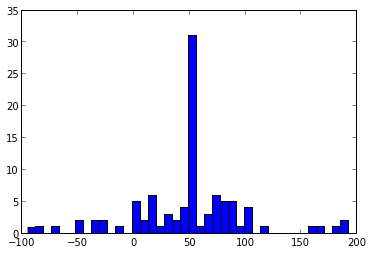
\includegraphics[width=0.7\textwidth]{stat_05_2_files/stat_05_2_fig_00.png}
\par
\end{center}
\end{codeoutput}
\end{codecell}
\begin{codecell}
\begin{codeinput}
\begin{lstlisting}
np.mean(data)
\end{lstlisting}
\end{codeinput}
\begin{codeoutput}
\begin{verbatim}
213.94889916666668
\end{verbatim}
\end{codeoutput}
\end{codecell}
\begin{codecell}
\begin{codeinput}
\begin{lstlisting}
np.median(data)
\end{lstlisting}
\end{codeinput}
\begin{codeoutput}
\begin{verbatim}
214.06
\end{verbatim}
\end{codeoutput}
\end{codecell}
\begin{codecell}
\begin{codeinput}
\begin{lstlisting}
np.std(data)
\end{lstlisting}
\end{codeinput}
\begin{codeoutput}
\begin{verbatim}
125.1184819538924
\end{verbatim}
\end{codeoutput}
\end{codecell}
\begin{codecell}
\begin{codeinput}
\begin{lstlisting}
np.mean(data)+2*np.std(data)
\end{lstlisting}
\end{codeinput}
\begin{codeoutput}
\begin{verbatim}
464.1858630744515
\end{verbatim}
\end{codeoutput}
\end{codecell}
\begin{codecell}
\begin{codeinput}
\begin{lstlisting}
np.percentile(data, 95)
\end{lstlisting}
\end{codeinput}
\begin{codeoutput}
\begin{verbatim}
410.41150000000005
\end{verbatim}
\end{codeoutput}
\end{codecell}
Goruldugu gibi uc nokta hesabi icin ortalamadan iki sapma otesini
kullanirsak, 464.18, fakat 95. yuzdeligi kullanirsak 410.41 elde
ediyoruz. Niye? Sebep ortalamanin kendisi hesaplanirken cok uc
degerlerin toplama dahil edilmis olmasi ve bu durum, ortalamanin
kendisini daha buyuk seviyeye dogru itiyor. Yuzdelik hesabi ise sadece
sayilari siralayip belli bazi elemanlari otomatik olarak uc nokta olarak
addediyor. Box Whisker Grafikleri

Tek boyutlu bir verinin dagilimini gormek icin Box ve Whisker grafikleri
faydali araclardir; medyan (median), dagilimin genisligini ve siradisi
noktalari (outliers) acik sekilde gosterirler. Isim nereden geliyor? Box
yani kutu, dagilimin agirliginin nerede oldugunu gosterir, medyanin
sagindada ve solunda olmak uzere iki ceyregin arasindaki kisimdir, kutu
olarak resmedilir. Whiskers kedilerin biyiklarina verilen isimdir, zaten
grafikte birazcik biyik gibi duruyorlar. Bu uzantilar medyan noktasindan
her iki yana kutunun iki kati kadar uzatilir sonra verideki ``ondan az
olan en buyuk'' noktaya kadar geri cekilir. Tum bunlarin disinda kalan
veri ise teker teker nokta olarak grafikte basilir. Bunlar siradisi
(outlier) olduklari icin daha az olacaklari tahmin edilir.

BW grafikleri iki veriyi dagilimsal olarak karsilastirmak icin
birebirdir. Mesela Larsen and Marx adli arastirmacilar cok az veri
iceren Quintus Curtius Snodgrass veri setinin degisik oldugunu
ispatlamak icin bir suru hesap yapmislardir, bir suru matematiksel
isleme girmislerdir, fakat basit bir BW grafigi iki setin farkliligini
hemen gosterir.

BW grafikleri iki veriyi dagilimsal olarak karsilastirmak icin
birebirdir. Mesela Larsen and Marx adli arastirmacilar cok az veri
iceren Quintus Curtius Snodgrass veri setinin degisik oldugunu
ispatlamak icin bir suru hesap yapmislardir, bir suru matematiksel
isleme girmislerdir, fakat basit bir BW grafigi iki setin farkliligini
hemen gosterir.

Python uzerinde basit bir BW grafigi

\begin{codecell}
\begin{codeinput}
\begin{lstlisting}
spread= rand(50) * 100
center = ones(25) * 50
flier_high = rand(10) * 100 + 100
flier_low = rand(10) * -100
data =concatenate((spread, center, flier_high, flier_low), 0)
plt.boxplot(data)
plt.show()

\end{lstlisting}
\end{codeinput}
\begin{codeoutput}
\begin{center}
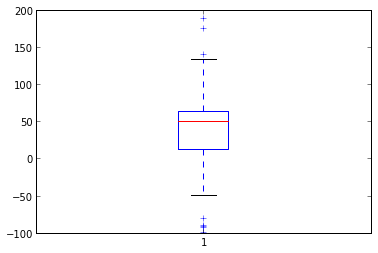
\includegraphics[width=0.7\textwidth]{stat_05_2_files/stat_05_2_fig_01.png}
\par
\end{center}
\end{codeoutput}
\end{codecell}
Bir diger ornek Glass veri seti uzerinde

\begin{codecell}
\begin{codeinput}
\begin{lstlisting}
data = loadtxt("glass.data",delimiter=",")
head = data[data[:,10]==7]
tableware = data[data[:,10]==6]
containers = data[data[:,10]==5]

print head[:,1]

data =(containers[:,1], tableware[:,1], head[:,1])

plt.yticks([1, 2, 3], ['containers', 'tableware', 'head'])

plt.boxplot(data,0,'rs',0,0.75)
plt.show()

\end{lstlisting}
\end{codeinput}
\begin{codeoutput}
\begin{verbatim}
[ 1.51131  1.51838  1.52315  1.52247  1.52365  1.51613  1.51602  1.51623
  1.51719  1.51683  1.51545  1.51556  1.51727  1.51531  1.51609  1.51508
  1.51653  1.51514  1.51658  1.51617  1.51732  1.51645  1.51831  1.5164
  1.51623  1.51685  1.52065  1.51651  1.51711]
\end{verbatim}
\begin{center}
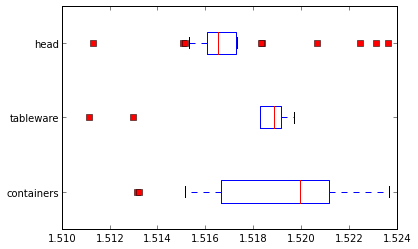
\includegraphics[width=0.7\textwidth]{stat_05_2_files/stat_05_2_fig_02.png}
\par
\end{center}
\end{codeoutput}
\end{codecell}
Guven Araligi (Confidence Intervals) Bu kavram istatistikte tartisilan
konulardan biri. Bayes ve Frenkansçı (Frequentist) istatistik arasindaki
felsefi farklardan biri burada ortaya cikiyor. Frekansci tanim soyledir:

"Bir parametre $\theta$ icin $1-\alpha$ seviyesinde bir $C_n=(a,b)$
guven araligi tanimlanabilir -- bu aralik $a=a(X_1,..,X_n)$ ve
$b=b(X_1,..,X_n)$ adli iki fonksiyon uzerinden tanimlanabilir. Bu
fonksiyonlar veri uzerinde isleyen, \emph{verinin} fonksiyonlaridir, ve
sonucta
\[ \mathbb{P}_\theta (\theta \in C_n) \ge 1-\alpha, \ \ \forall \theta \in \Theta \]
Yani $(a,b)$ araligi $1-\alpha$ olasiliginda $\theta$ 'yi icine alir /
hapseder.

Daha detayli olarak deney arka arkaya pek cok kez tekrarlandiginda
parametrenin tahmininin $1-\alpha$ oraninda tanimlanan araliga dusecegi
soylenir. $1-\alpha$ sayisina guven araliginin kapsami (coverage) ismi
de verilir. Genellikle insanlar yuzde 95 guven araligini kullanirlar, ve
bu yuzdeye tekabul eden $\alpha = 0.05$ rakami kullanilir.

Uzerine basarak belirtmek gerekir ki $C_n$ rasgele (random) bir
degerdir, ama $\theta$ sabittir, cunku $C_n$ verinin bir fonksiyonudur,
ve veriden, yani bir orneklemden gelecegi icin o da rasgele olmalidir.

Eger $\theta$ bir vektor ise o zaman bir aralik yerine bir guven kumesi
kullanilir (mesela bir kure, ya da elips). "
Fakat frekansci yaklasimda aralik fonksiyonlari $a,b$ ile guven araligi
arasindaki baglanti net degildir. Hangi fonksiyon secimi hangi
$\alpha$'ya sebebiye vermektedir? Bu durum net oldugu durumlarda bile
teorik olarak saglamligi suphelidir, ayrica hesabin sozel olarak ortaya
konmasinda bazi eksikler vardir. ``Deney arka arkaya pek cok kez
tekrarlandiginda parametrenin tahmini, $1-\alpha$ guven araliga
dusecektir'' ibaresi mesela; ``deney tekrari'' her durumda gecerli
olmayabilir. Meteoroloji ``yarin yuzde 80 ihtimali ile yagmur yagacak''
diyorsa, o hesap sartlarinin bir daha ortaya cikmasinin olasiligi cok
dusuktur, Kaos Teorisi bize en azindan bunu soyluyor.

Wiki sayfasinda {[}1{]} tartismanin boyutlari gorulebilir.

Son onyillarda ortaya cikan yaklasim ise Bayes Teorisini devreye sokmak.
Bir guven araligi tanimlamanin en saglam yolu bu hesabi bir dagilimi baz
alarak yapmak. Eger sonuc olarak bir tekil sayi degil, bir dagilim elde
edersek bu dagilim uzerinde guvenlik hesaplarini yapmak cok kolay hale
gelir. Mesela sonuc (sonsal dagilim) bir Gaussian dagilim ise, bu
dagilimin yuzde 95 agirliginin nerede oldugu, ve nasil hesaplandigi
bellidir.

Bayes Teorisi
\[ P(A|B)  = \frac{ P(B|A)P(A)}{P(B)} \]
Veri analizi baglaminda diyelim ki deneyler yaparak tahmini olarak
hesaplamak (estimate) istedigimiz bir parametre var, bu bir protonun
kutlesi ya da bir ameliyat sonrasi hayatta kalma orani olabilir. Bu
durumlarda iki ayri ``olaydan'' bahsetmemiz gerekir, B olayi spesifik
bazi olcumlerin elde edilmesi ``olayidir'', mesela olcum uc sayidan
olusuyorsa, biz bir olcumde spesifik olarak $\{0.2,4,5.4\}$ degerlerini
elde etmisiz. Ikinci olay bilmedigimiz parametrenin belli bir degere
sahip olmasi olacak. O zaman Bayes Teorisinin su sekilde tekrar
yazabiliriz,
\[ P(parametre | veri ) \propto P(data | parametre)P(parametre) \]
$\propto$ isareti orantili olmak (proportional to) anlamina geliyor.
Boleni attik cunku o bir sabit (tamamen veriye bagli, tahmini hesaplamak
istedigimiz parametreye bagli degil). Tabii bu durumda sol ve sag taraf
birbirine esit olmaz, o yuzden esitlik yerine orantili olmak isaretini
kullandik. Bu cercevede ``belli bir numerik sabit cercevesinde birbirine
esit (equal within a numeric constant)'' gibi cumleler de gorulebilir.

Ornek

Diyelim ki bir bozuk para ile 10 kere yazi-tura attik, ve sonuc altta

T H H H H T T H H H

Bu veriye bakarak paranin hileli olup olmadigini anlamaya calisacagiz.
Bayes ifadesini bu veriye gore yazalim,
\[ P(p | \{ \textrm{T H H H H T T H H H} \} \propto 
P(\{ \textrm{T H H H H T T H H H} | p) P(p) \}
\]
$P(p)$ ifadesi ne anlama gelir? Aslinda bu ifadeyi $P([Dagilim] = p)$
olarak gormek daha iyi, artik $p$ parametresini bir dagilimdan gelen bir
tekil deger olarak gordugumuze gore, o dagilimin belli bir $p$'ye esit
oldugu zamani modelliyoruz burada. Her halukarda $P(p)$ dagilimini, yani
onsel (prior) olasiligi bilmiyoruz, hesaptan once her degerin mumkun
oldugunu biliyoruz, o zaman bu onsel dagilimi duz (flat) olarak aliriz,
yani $P(p) = 1$.

$P(\{\textrm{T H H H H T T H H H} | p)$ ifadesi goz korkutucu olabilir,
ama buradaki her ogenin bagimsiz ozdesce dagilmis (independent
identically distributed) oldugunu gorursek, ama bu ifadeyi ayri ayri
$P(\{\textrm{T}|p)$ ve $P(\{\textrm{H}|p)$ carpimlari olarak
gorebiliriz. $P(\{\textrm{T}|p) = p$ ve $P(\{\textrm{H}|p)=1-p$ oldugunu
biliyoruz. O zaman
\[ P(p | \{ \textrm{7 Tura, 3 Yazi} \} \propto
p^7(1-p)^3
\]
Grafiklersek,

\begin{codecell}
\begin{codeinput}
\begin{lstlisting}
im=imread("05_01.png"); imshow(im)
\end{lstlisting}
\end{codeinput}
\begin{codeoutput}
\begin{verbatim}
<matplotlib.image.AxesImage at 0xb32ffec>
\end{verbatim}
\begin{center}
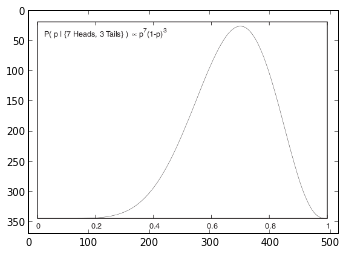
\includegraphics[width=0.7\textwidth]{stat_05_2_files/stat_05_2_fig_03.png}
\par
\end{center}
\end{codeoutput}
\end{codecell}
Boylece $p$ icin bir sonsal (posterior) dagilim elde ettik. Artik bu
dagilimin yuzde 95 agirliginin nerede oldugunu rahatca gorebiliriz /
hesaplayabiliriz. Dagilimin tepe noktasinin $p=0.7$ civarinda oldugu
goruluyor. Bir dagilimla daha fazlasini yapmak ta mumkun, mesela bu
fonksiyonu $p$'ye bagli baska bir fonksiyona karsi entegre etmek mumkun,
mesela beklentiyi bu sekilde hesaplayabiliriz.

Onsel dagilimin her noktaya esit agirlik veren birornek (uniform)
secilmis olmasi, yani problemi cozmeye sifir bilgiden baslamis olmamiz,
yontemin bir zayifligi olarak gorulmemeli. Yontemin kuvveti elimizdeki
bilgiyle baslayip onu net bir sekilde veri ve olurluk uzerinden sonsal
tek dagilima goturebilmesi. Baslangic ve sonuc arasindaki baglanti gayet
net. Fazlasi da var; ilgilendigimiz alani (domain) ogrendikce, basta hic
bilmedigimiz onsel dagilimi daha net, bilgili bir sekilde secebiliriz ve
bu sonsal dagilimi da daha olmasi gereken modele daha yaklastirabilir.

Gaussian Kontrolu

Diyelim ki Gaussian dagilimina sahip oldugunu dusundugumuz $\{ x_i\}$
verilerimiz var. Bu verilerin Gaussian dagilimina uyup uymadigini nasil
kontrol edecegiz? Normal bir dagilimin her veri noktasi icin soyle
temsil edebiliriz,
\[ y_i = \Phi\bigg(\frac{ x_i - \mu}{\sigma}\bigg) \]
Burada $\Phi$ standart Gaussian'i temsil ediyor (detaylar icin
\emph{Istatistik Ders 1}) ve CDF fonksiyonuna tekabul ediyor. CDF
fonksiyonunun ayni zamanda ceyregi (quantile) hesapladigi soylenir,
aslinda CDF son derece detayli bir olasilik degeri verir fakat evet,
dolayli yoldan noktanin hangi ceyrek icine dustugu de gorulecektir.

Simdi bir numara yapalim, iki tarafa ters Gaussian formulunu
uygulayalim, yani $\Phi^{-1}$.
\[ \Phi^{-1}(y_i) = \Phi^{-1}\bigg( \Phi\bigg(\frac{ x_i - \mu}{\sigma}\bigg)\bigg) \]\[ \Phi^{-1}(y_i) = \frac{ x_i - \mu}{\sigma}\]\[ x_i = \Phi^{-1}(y_i) \sigma + \mu  \]
Bu demektir ki elimizdeki verileri $\Phi^{-1}(y_i)$ bazinda
grafiklersek, bu noktalar egimi $\sigma$, baslangici (intercept) $\mu$
olan bir duz cizgi olmalidir. Eger kabaca noktalar duz cizgi
olusturmuyorsa, verimizin Gaussian dagilima sahip olmadigina karar
verebiliriz.

Ustte tarif edilen grafik, olasilik grafigi (probability plot) olarak
bilinir.

Ters Gaussian teorik fonksiyonunu burada vermeyecegiz, Scipy
\verb!scipy.stats.invgauss! hesaplar icin kullanilabilir. Fakat
$y_i$'nin kendisi nereden geliyor? Eger $y_i$, CDF'in bir sonucu ise,
pur veriye bakarak bir CDF degeri de hesaplayabilmemiz gerekir. Bunu
yapmak icin bir baska numara lazim.

\begin{enumerate}[1.]
\item
  Eldeki sayilari artan sekilde siralayin
\item
  Her veri noktasina bir derece (rank) atayin (siralama sonrasi hangi
  seviyede oldugu yeterli, 1'den baslayarak).
\item
  Ceyrek degeri $y_i$ bu sira / $n+1$, $n$ eldeki verinin buyuklugu.
\end{enumerate}
Bu teknik niye isliyor? $x$'in CDF'i $x_i < x$ sartina uyan $x_i$'lerin
orani degil midir? Yani bir siralama soz konusu ve ustteki teknik te bu
siralamayi biz elle yapmis olduk, ve bu siralamadan gereken bilgiyi
aldik.

Kaynaklar

{[}1{]} http://en.wikipedia.org/wiki/Confidence\_interval

{[}2{]} Janert, P., Data Analysis with Open Source Tools

\end{document}
